\documentclass{beamer}

\newcommand{\lesson}{JavaFX GUIs}


\newcommand{\course}{Introduction to Object-Oriented Programming}
\subject{\course}
\title[\lesson]{\course}
\subtitle{\lesson}

\author[CS 1331]
{Christopher Simpkins \\\texttt{chris.simpkins@gatech.edu}}
\institute[Georgia Tech]

\date[]{}

\newcommand{\link}[2]{\href{#1}{\textcolor{blue}{\underline{#2}}}}
\newcommand{\code}{http://www.cs1331.org/code}

\usepackage{colortbl}

% If you have a file called "university-logo-filename.xxx", where xxx
% is a graphic format that can be processed by latex or pdflatex,
% resp., then you can add a logo as follows:

% \pgfdeclareimage[width=0.6in]{coc-logo}{cc_2012_logo}
% \logo{\pgfuseimage{coc-logo}}

\mode<presentation>
{
  \usetheme{Berlin}
  \useoutertheme{infolines}

  % or ...

 \setbeamercovered{transparent}
  % or whatever (possibly just delete it)
}

\usepackage{tikz}
% Optional PGF libraries
\usepackage{pgflibraryarrows}
\usepackage{pgflibrarysnakes}
\usepackage{pgfplots}
\usepackage{fancybox}
\usepackage{listings}
\usepackage{hyperref}
\hypersetup{colorlinks=true,urlcolor=blue}
\usepackage[english]{babel}
% or whatever

\usepackage[latin1]{inputenc}
% or whatever

\usepackage{times}
\usepackage[T1]{fontenc}
% Or whatever. Note that the encoding and the font should match. If T1
% does not look nice, try deleting the line with the fontenc.


\usepackage{listings}

% "define" Scala
\lstdefinelanguage{scala}{
  morekeywords={abstract,case,catch,class,def,%
    do,else,extends,false,final,finally,%
    for,if,implicit,import,match,mixin,%
    new,null,object,override,package,%
    private,protected,requires,return,sealed,%
    super,this,throw,trait,true,try,%
    type,val,var,while,with,yield},
  otherkeywords={=>,<-,<\%,<:,>:,\#,@},
  sensitive=true,
  morecomment=[l]{//},
  morecomment=[n]{/*}{*/},
  morestring=[b]",
  morestring=[b]',
  morestring=[b]""",
}

\usepackage{color}
\definecolor{dkgreen}{rgb}{0,0.6,0}
\definecolor{gray}{rgb}{0.5,0.5,0.5}
\definecolor{mauve}{rgb}{0.58,0,0.82}

% Default settings for code listings
\lstset{frame=tb,
  language=scala,
  aboveskip=2mm,
  belowskip=2mm,
  showstringspaces=false,
  columns=flexible,
  basicstyle={\scriptsize\ttfamily},
  numbers=none,
  numberstyle=\tiny\color{gray},
  keywordstyle=\color{blue},
  commentstyle=\color{dkgreen},
  stringstyle=\color{mauve},
  frame=single,
  breaklines=true,
  breakatwhitespace=true,
  keepspaces=true
  %tabsize=3
}


% \beamerdefaultoverlayspecification{<+->}

\begin{document}

\begin{frame}
  \titlepage
\end{frame}


%------------------------------------------------------------------------
\begin{frame}[fragile]{Todo GUI}

Today we'll make a GUI for todo lists
\begin{center}
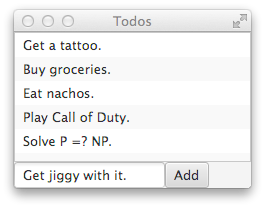
\includegraphics[height=1.5in]{javafx-todo.png}
\end{center}

Along the way we'll
\begin{itemize}
\item Review event handling
\item Learn two new UI controls
\item Learn about nested layouts
\item See an example of MVC in JavaFX
\item See a basic use of JavaFX's properties
\end{itemize}


\end{frame}
%------------------------------------------------------------------------

%------------------------------------------------------------------------
\begin{frame}[fragile]{The Application}
Where do we start?  The {\tt Application}:
\begin{lstlisting}[language=Java]
import javafx.application.Application;
import javafx.stage.Stage;

public class TodoList extends Application {

    @Override public void start(Stage stage) {

    }
}
\end{lstlisting}

And now we just follow our recipe:
\begin{itemize}
\item Create UI controls
\item Add UI controls to a parent node in a scene graph
\item Set the stage's scene graph and show
\end{itemize}


\end{frame}
%------------------------------------------------------------------------

%------------------------------------------------------------------------
\begin{frame}[fragile]{Create UI Controls}

\begin{lstlisting}[language=Java]
    @Override public void start(Stage stage) {
        ListView<String> listView = new ListView<String>();

        Button addButton = new Button();
        addButton.setText("Add");

        TextField inputField = new TextField();
    }
\end{lstlisting}
And, of course, we'll need to import these:
\begin{lstlisting}[language=Java]
import javafx.scene.control.Button;
import javafx.scene.control.ListView;
import javafx.scene.control.TextField;
\end{lstlisting}



\end{frame}
%------------------------------------------------------------------------

%------------------------------------------------------------------------
\begin{frame}[fragile]{Add UI Controls to Parent Node - Layout}


\begin{center}
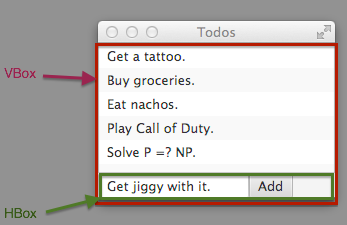
\includegraphics[height=1.5in]{javafx-todo-nesting.png}
\end{center}

To acheive the layout we want, we'll nest an {\tt HBox} inside a {\tt VBox}:
\begin{lstlisting}[language=Java]
    @Override public void start(Stage stage) {
        HBox entryBox = new HBox();
        entryBox.getChildren().addAll(inputField, addButton);

        VBox vbox = new VBox();
        vbox.getChildren().addAll(listView, entryBox);
    }
\end{lstlisting}

\end{frame}
%------------------------------------------------------------------------

%------------------------------------------------------------------------
\begin{frame}[fragile]{Setting up and showing the stage}

Although we're not done with our UI controls, we go ahead and do the last step of our recipe so we can run the program:

\begin{lstlisting}[language=Java]
import javafx.scene.Scene;
// ...

public class TodoList extends Application {
    @Override public void start(Stage stage) {
        // ...
        Scene scene = new Scene(vbox);
        stage.setScene(scene);
        stage.setTitle("Todos");
        stage.show();
    }
}
\end{lstlisting}


\end{frame}
%------------------------------------------------------------------------


%------------------------------------------------------------------------
\begin{frame}[fragile]{The Model-View-Controller Design Pattern}
\vspace{-.1in}
\begin{center}
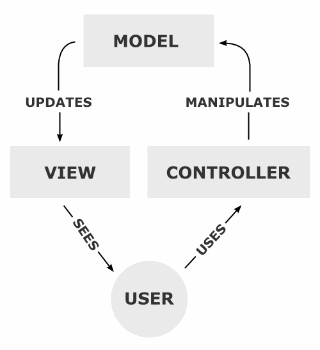
\includegraphics[height=1.5in]{MVC-Process.png}\footnote{\url{http://en.wikipedia.org/wiki/File:MVC-Process.png}}
\end{center}
\vspace{-.1in}
\begin{itemize}
\item The {\it model} contains the data that is displayed by the {\it view}
\item The {\it view} displays the data from the {\it model} on screen
\item The {\it controller} gets input from the user and manipulates the model
\end{itemize}
In JavaFX the view and controller are typically combined.

\end{frame}
%------------------------------------------------------------------------


%------------------------------------------------------------------------
\begin{frame}[fragile]{ListView, ObservableList, and MVC}

JavaFX provides model classes that work with UI controls.  For our {\tt ListView} we'll simply use an {\tt ObservableList<String>}, which we obtain from {\tt FXCollections.observableArrayList()}:
\begin{lstlisting}[language=Java]
import javafx.collections.FXCollections;
import javafx.collections.ObservableList;

public class TodoList extends Application {

    private ObservableList<String> todos;

    @Override public void start(Stage stage) {
        ObservableList<String> todos = FXCollections.observableArrayList();
        ListView<String> listView = new ListView<String>(todos);
        // ...
\end{lstlisting}


\end{frame}
%------------------------------------------------------------------------

%------------------------------------------------------------------------
\begin{frame}[fragile]{Handling Model Updates}

\begin{itemize}
\item Whenever the {\tt ObservableList<String> todos} is updated, the change is automatically reflected in the {\tt ListView}.
\item So all we have to do is add text from the {\tt TextField} to the {\tt todos} list whenever the add button is clicked.
\end{itemize}

\begin{lstlisting}[language=Java]
    @Override public void start(Stage stage) {
        // ...
        addButton.setOnAction(e -> {
            todos.add(inputField.getText());
            inputField.setText("");
            inputField.requestFocus();
        });
        // ...
    }
\end{lstlisting}

Notice that after the text is added to the list we reset the text field and give it the focus again.

\end{frame}
%------------------------------------------------------------------------

%------------------------------------------------------------------------
\begin{frame}[fragile]{Properties}

We don't want to add empty strings from the TextField to the todos list, so let's disable the Add button when the TextField is empty:

\begin{lstlisting}[language=Java]
import javafx.beans.binding.Bindings;
// ...

public class TodoList extends Application {

    private ObservableList<String> todos;

    @Override public void start(Stage stage) {
        // ...
        addButton.disableProperty()
            .bind(Bindings.isEmpty(inputField.textProperty()));
        // ...
    }
}
\end{lstlisting}

Properties play a big role in modern JavaFX programming.  This is just a small taste.

\end{frame}
%------------------------------------------------------------------------


%------------------------------------------------------------------------
\begin{frame}[fragile]{Conclusion}

Very simple app to get started with UI controls and MVC.
\begin{itemize}
\item GUI programming requires two things:
\begin{itemize}
  \item Knowledge of GUIs (widgets, how they work, how they're used)
  \item Knowledge of a particular GUI framework (like JavaFX)
\end{itemize}
\item The JavaFX classes you've seen make extensive use of OOP.
\item GUI programs are straightforward, but get complex quickly.
\item JavaFX's properties and the Model-View-Controller pattern help us deal with the complexity of GUI programming.
\end{itemize}

The full Todos example is online: \link{\code/javafx/TodoList.java}{TodoList.java}.

\end{frame}
%------------------------------------------------------------------------


% %------------------------------------------------------------------------
% \begin{frame}[fragile]{}

% \begin{itemize}
% \item
% \end{itemize}

% \begin{lstlisting}[language=Java]

% \end{lstlisting}


% \end{frame}
% %------------------------------------------------------------------------

\end{document}
